% StoneKit manuscript (IEEE conference format). Stage B redesign, 14 November 2026.
% Every number traces to docs/results.md and a results/runs/<folder>; T1 numbers come from
% results/runs/T1_20261113T081425Z/analysis/evaluation.json and external numbers from
% results/runs/mswal_external_check_20261113T132418Z/external_check.json.
% Figures: scripts/make_paper_figures.py (reads only hashed result artefacts; writes a data CSV per figure).
\documentclass[conference]{IEEEtran}
\usepackage{amsmath,amssymb}
\usepackage{booktabs}
\usepackage{graphicx}
\usepackage{xcolor}
\usepackage{siunitx}
\usepackage{cite}
\usepackage{url}
\usepackage{flushend} % balances the two columns on the last page
\input{glyphtounicode}\pdfgentounicode=1 % correct text extraction from the PDF
\newcommand{\pending}[1]{\textcolor{red}{[PENDING: #1]}}


\makeatletter
\def\@IEEEauthorblockNstyle{\normalfont\small}
\def\@IEEEauthorblockAstyle{\normalfont\footnotesize}
\makeatother


% --- layout only: tighter float and display spacing ---
\setlength{\textfloatsep}{6pt plus 2pt minus 2pt}
\setlength{\floatsep}{6pt plus 2pt minus 2pt}
\setlength{\intextsep}{6pt plus 2pt minus 2pt}
\setlength{\dbltextfloatsep}{6pt plus 2pt minus 2pt}
\setlength{\dblfloatsep}{6pt plus 2pt minus 2pt}
\setlength{\abovecaptionskip}{1pt}
\setlength{\belowcaptionskip}{0pt}
\AtBeginDocument{\setlength{\abovedisplayskip}{5pt}\setlength{\belowdisplayskip}{5pt}\setlength{\abovedisplayshortskip}{4pt}\setlength{\belowdisplayshortskip}{4pt}}

\begin{document}
\bstctlcite{IEEEexample:BSTcontrol}

\title{Detection-Aware Conformal Uncertainty for Automated Kidney-Stone Measurement on Non-Contrast CT}

\author{\IEEEauthorblockN{Dr.~Suresh Kumar Kanaparthi}
\IEEEauthorblockA{\textit{Department of Computer Science}\\
\textit{and Engineering}\\
\textit{SRM University-AP, Amaravati}\\
\textit{522 240, Andhra Pradesh, India.}\\
sureshkumar.k@srmap.edu.in\\
\textit{(Corresponding author)}}
\and
\IEEEauthorblockN{Abhijith Reddy Kadari}
\IEEEauthorblockA{\textit{Department of Computer Science}\\
\textit{and Engineering}\\
\textit{SRM University-AP, Amaravati}\\
\textit{522 240, Andhra Pradesh, India.}\\
abhijithreddy2006@gmail.com}
\and
\IEEEauthorblockN{Sai Praneeth Surepalli}
\IEEEauthorblockA{\textit{Department of Computer Science}\\
\textit{and Engineering}\\
\textit{SRM University-AP, Amaravati}\\
\textit{522 240, Andhra Pradesh, India.}\\
praneethh777@gmail.com}
\and
\IEEEauthorblockN{Jaswanth Kolisetty}
\IEEEauthorblockA{\textit{Department of Computer Science}\\
\textit{and Engineering}\\
\textit{SRM University-AP, Amaravati}\\
\textit{522 240, Andhra Pradesh, India.}\\
kolisettyjaswanth8@gmail.com}}

\maketitle

\begin{abstract}
Automated kidney-stone volumetry in CT has been commonly assessed through the use of agreement statistics, which are not able to provide a deep insight into the errors associated with the volumetric assessment of individual stones as well as missed stones or false positive stones. We introduced the concept of calibrated intervals in two stages in the automated pipeline levels characterized by the use of per-stone volume intervals and three-dimensional diameter intervals calibrated for every stone size. In addition, we included a patient-level burden interval combining false positive probability, volume measurement residuals for identified stones and missed burden before one conformal calibration stage. To our knowledge, this is the first calibrated interval for kidney-stone burden that represents missed and false detections. Results were obtained once from 53 locked test cases, after calibration on 35 cases under a protocol frozen in advance. At nominal level of 0.90, the burden interval allowed to cover 50 out of 53 cases even being narrower than the conformal quantile regression based interval that provided a similar level of coverage (paired median width ratio 0.573; 95\% CI 0.540--0.656) and using the pre-specified kidney distance filter; without the filter, the widths of the two intervals did not clearly differ. The size-based diameter intervals were able to cover 29 out of 31 stones predicted below 5\,mm, against 19 of 31 for a global interval. On 58 scans of an independent dataset, with nothing refitted, burden coverage held (56 of 58), but the width advantage did not transfer and per-stone volume intervals under-covered (0.733). On a phantom with physical reference volumes, an ICC of 0.993 coexisted with a 23.6\% median per-stone volume error. On the same phantom, 7 stones were placed in the correct 10\,mm category only by 3D diameter and none only by 2D (exact McNemar $p=0.016$).
\end{abstract}

\begin{IEEEkeywords}
kidney stone, computed tomography, conformal prediction, uncertainty quantification, volumetry, external evaluation
\end{IEEEkeywords}

\section{Introduction}
The measurement of size and burden of the stone is a fundamental metric for urolithiasis and the development of deep segmentation systems that allow for the automatic measurement of 3D stone volume is now a possibility, as shown in previous studies \cite{elton2022,li2022,cumpanas2024,mukherjee2023}. These systems usually rely on the coefficients of correlation or the Intraclass Correlation Coefficient (ICC) for validation against some reference value \cite{neubauer2023,wilhelm2018,elton2022}. Since the variation in stone volume is quite large, the differences between stones are mainly responsible for the ICC value. These statistics can stay close to 1 even when individual stones are measured poorly; the same effect has been reported for small lung nodules \cite{xie2013}. When we test the public phantom with water-displacement volume, we saw that there is an ICC of 0.993, whereas the median error per stone is 23.6\%, and 7 stones reach the correct 10\,mm category only by 3D diameter (Section~\ref{sec:res_phantom}). As far as the patient burden is concerned, other sources of error are also present and not covered by the agreement statistics: those stones that were missed by the model and those pieces that were detected but are not stones.

Thus a person wishing to make use of the automated measurement system requires an uncertainty measure for each detected stone and stone burden which will be applicable to new scans. The split conformal prediction provides a person with the possibility to have finite-sample marginal coverage at a defined level when calibration and test data are exchangeable \cite{vovk2005,romano2019}; whether that assumption holds has to be checked on real data. Conformal intervals already exist for volumes derived from segmentation \cite{lambert2024,alijani2026,jaubert2025}, but they cover the total volume of one structure and cannot represent missed or spurious objects. Burden error has been split into matched, missed and false-positive components \cite{kataria2026}, but only descriptively, not as a calibrated interval. For kidney stones, conformal prediction has been used for slice-level classification \cite{obeten2026}. To our knowledge, no conformal research has been done regarding either the stone size or burden.

\textbf{Contributions.} (i) A patient-level burden interval that takes into account false positives, measurement error of stones stratified by size, and undetected burden, with one conformal calibration on top. In a single locked evaluation at nominal 0.90, the median ratio of widths per scan to the direct conformalised quantile-regression interval was 0.573, so it was at least 42.7\% narrower in at least half of the scans at similar coverage. The kidney distance filter stands as a condition for this result. (ii) Evidence, rather than a new algorithm, that size-stratified (Mondrian) stone intervals provide better coverage for small stones compared to a global conformal interval, evident first in developmental data and then in held out data. (iii) A descriptive verification of the unchanged system on an independent data set, stating what was applicable and what was not. (iv) An open implementation, including a local workstation, that applies frozen calibration to new scans.

\section{Related Work}\label{sec:related}
\textbf{Automated Stone Measurement.} Deep learning has been used to detect and segment stones in non-contrast CT to determine volume or burden \cite{elton2022,li2022,cumpanas2024,mukherjee2023}; the results are validated through the agreement with either manual or semi-manual means \cite{wilhelm2018,neubauer2023}. Phantom research is presented to demonstrate how the error is influenced by the thickness of slices and composition of stones \cite{thongprayoon2026,neubauer2023}. 2D measurements underestimate the stones that are not aligned with the picture planes so that stones appear in another size category \cite{liden2015,berkovitz2010}, and manual measurements prove to be the most effective on multiplanar images \cite{reimer2021}. From the research revealed, we see that there were no calibrated intervals reported either for a particular stone or the burden.

\textbf{Uncertainty in the amount of segmentation-derived objects.} Available methods include Monte Carlo error bars \cite{eatonrosen2018}, conformal volume intervals considering the change of covariates \cite{lambert2024}, asymmetric conformal volume based on class awareness \cite{alijani2026}, and volume conditional coverage for the volume of coronary calcium \cite{jaubert2025}; all of them are committed to measuring the total volume of a structure. Patient-level conformal intervals for PSMA tumour volume may be found in \cite{psmatv2026}, and the amount of a tumour missed by segmentation is reported as a per-case bound with a conformal guarantee \cite{vargas2026}. Work on lesion-level uncertainty points out that a missed lesion gets no uncertainty estimate at all \cite{molchanova2025}. For lung nodules, repeatability-based 95\% intervals exist for single nodule volumes \cite{qiba2023nodule}, but they are not calibrated against a reference on held-out data.

\textbf{Conformal building blocks.} All the conformal tools we use are established: split conformal prediction, its category-conditional (Mondrian) form \cite[Sec.~4.5]{vovk2005}, conformalised quantile regression \cite{romano2019} and joint coverage of all objects in an image \cite{andeol2025}. What we add is how they are combined with detection modelling for stone burden, and the locked and external evaluation of that combination.




\section{Methodology}
\begin{figure*}[t]
\centering
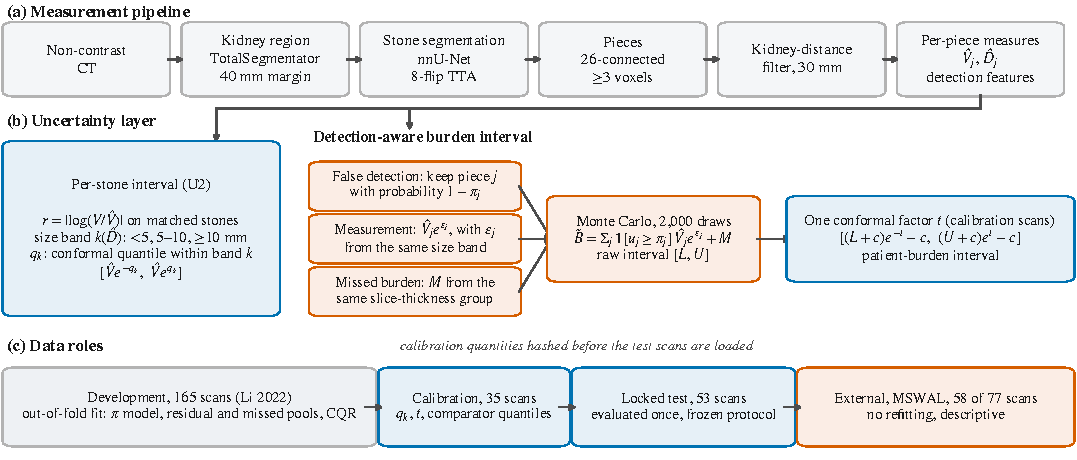
\includegraphics[width=0.567\textwidth]{figures/fig1_overview.pdf}
\caption{Overview of StoneKit. (a): measurement pipeline; (b): uncertainty layer: size-stratified per-stone interval (1) and detection-aware burden interval (2 to 4) propagate false detection probabilities $\pi_j$, size-band residuals $\varepsilon_j$ and missed burden $M$ prior to one conformal calibration; (c): data roles: model components are fitted to out-of-fold development data and each conformal quantity to separate calibration scans; locked test and external scans are used only for evaluation.}
\label{fig:overview}
\end{figure*}

\subsection{Data}
\textbf{Patient CT.} We utilize the Li dataset \cite{li2022} from 2022 in this study, which offers 260 CT scans from a certain hospital that have been obtained without any contrast. The scans have expert kidney stone annotations. The expert masks are used as the reference standard, although they cannot be trusted as the actual truth. After conducting the audit rule, we are left with 253 scans that are split, before any model development, into 165 for development, 35 for calibration, and 53 for testing purposes. The calibration and testing scans cannot be loaded before confirmation run. As there are no identifiers with the patients, we had to do our own audit through images for repeats. We found 12 suspected repeat scans (6 calibration and 6 tests) that pair with a scan in another split, as well as 3 development pairs that fall across the training/validation boundary of the deployed fold. The thickness of original CT slice is somewhere between 0.42\,mm and 2.5\,mm. \textbf{External data.} We also use the MSWAL \cite{wu2026mswal} (CC BY-NC 4.0) dataset, with 484 abdominal CT scans and a total of 77 scans with labelled kidney stones (300 annotated components) and no phase label. Using the values obtained, we use aortic attenuation checking to identify non-contrast scans (median less than 100\,HU). \textbf{Physical reference.} The Freiburg set \cite{neubauer2023} (CC BY 4.0) has 101 ex-vivo stones scanned in a water phantom (100\,kVp, 0.7\,mm slices), with water-displacement volume, mean caliper diameter and, for 59 stones, composition.

\subsection{Measurement pipeline}
CT images are processed in RAS orientation without remapping (Fig.~\ref{fig:overview}a). TotalSegmentator 2.18.0 \cite{wasserthal2023} is used for the segmentation of kidneys, and cropping is done for a 40\,mm region around the kidneys. The segmentation of stones is carried out with nnU-Net v2 2.8.1 \cite{isensee2021} implementation (3D full resolution, 100 epochs). Here, test-time augmentation (TTA) is applied with eight-flip augmentation. A piece (candidate connected component) is defined as a group of voxels that are 26-connected with each other with at least three voxels in total. The piece filter, which is specified earlier, limits the detection of pieces to a maximum of 30\,mm from a kidney. The 30\,mm value was set from development annotations before any filter results existed (95th percentile of the farthest stone-label distance, rounded up). The measurements include both the voxel volume $\hat V$ and maximum diameter $\hat D$ (the largest distance between voxel centres) of a connected component. The diameter is measured in 3D because of the results obtained in Section~\ref{sec:res_phantom}. The processing has been carried out with 154 development scans that have been used for five-fold cross-validations. Each of them has an out-of-fold (OOF) prediction; the remaining 11 development scans were predicted by a model not trained on them. All uncertainty components are fitted on these OOF predictions. On the OOF predictions, 66\% of the annotated stones were found (95\% CI 59.0--73.8\%; false positives are in Table~\ref{tab:external}).

\subsection{Per-stone intervals}
We link annotated and predicted pieces when their voxels overlap. A linked group with exactly one annotated and one predicted piece is a one-to-one match. An annotated piece with no overlap is missed; a predicted piece with no overlap is a false positive. The absolute value of log ratio $r=|\log(V/\hat V)|$ gives the overall score and $D$ is measured in a similar way. It means that the match should be classified in size brackets $k(\hat D)\in\{{<}5,\,5\text{--}10,\,{\ge}10\}$\,mm. The size-stratified (Mondrian) interval is formed using only calibration stones from the same band:
\begin{equation}
\hbox{\small$\displaystyle q_k=\mathrm{Q}_{\lceil (n_k+1)(1-\alpha)\rceil/n_k}\bigl\{r_i : k(\hat D_i)=k\bigr\},\quad
\bigl[\hat V e^{-q_k},\ \hat V e^{q_k}\bigr],$}
\end{equation}
where $\mathrm{Q}_p$ is an empirical $p$-quantile, $n_k$ is the number of stones in calibration band $k$. If one of the bands has fewer than 20 calibration stones, it is joined with a neighbour. We compared against Bland--Altman log limits (U0) and global split conformal (U1). The selection rule, fixed on development data, required every band's Clopper--Pearson lower bound to reach nominal $-0.05$. No method met it, so the Mondrian interval (U2) was kept as pre-specified. We also report an interval scaled by each stone's TTA spread (U4), but only as an exploratory comparator.

\subsection{Detection-aware burden interval}
Assume $B$ denotes the annotated burden of the patient and $\hat V_j$ shows the volumes of the kept items. The logistic model fitted on the OOF development items provides the probability of a false detection $\pi_j$ for each item, while the inputs for the model are such parameters as the log volume, average segmentation probability, distribution of TTA, threshold sensitivity, distance to the kidney, and attenuation. For $d=1,\dots,2000$ we further construct
\begin{equation}
\hbox{\small$\displaystyle \tilde B^{(d)}=\sum_j \mathbf{1}\bigl[u_j^{(d)}\ge \pi_j\bigr]\,\hat V_j\,e^{\varepsilon_j^{(d)}}+M^{(d)},$}
\end{equation}
where $u_j^{(d)}\sim U(0,1)$, $\varepsilon_j^{(d)}$ is sampled from the development log residuals of the identical size band, while $M^{(d)}$ is sampled from the development missed burden for each scan and every group having the same slice thickness. The $\alpha/2$ quantiles and $1-\alpha/2$ quantiles produce a raw interval $[L,U]$. Then on the $n$ calibration scans we compute
\begin{equation}
\hbox{\small$\displaystyle s=\max\Bigl\{\log\tfrac{L+c}{B+c},\ \log\tfrac{B+c}{U+c}\Bigr\},\quad t=\mathrm{Q}_{\lceil (n+1)(1-\alpha)\rceil/n}\{s\},$}
\end{equation}
with $c=5$\,mm$^3$, and report
\begin{equation}
\hbox{\small$\displaystyle \bigl[\max\{(L+c)e^{-t}-c,\,0\},\ (U+c)e^{t}-c\bigr].$}
\end{equation}
Here we get only $t$ calibrated, while $\pi$, missed burden pool, and residual pool are all based on the development data. We are making comparisons with three approaches: naive sum of per-piece Mondrian bounds (P2-0); an interval obtained using direct split conformalization of $|\log((B+c)/(\hat B+c))|$, with $\hat B=\sum_j \hat V_j$ (P2-B); and CQR \cite{romano2019} of $\log(B+c)$ on $\log(\hat B+c)$, the false-positive-adjusted volume and slice thickness (P2-B-CQR), going through the entire development process with CQR being the best method in comparison with the other comparators in development.

\begin{figure}[tb]
\centering
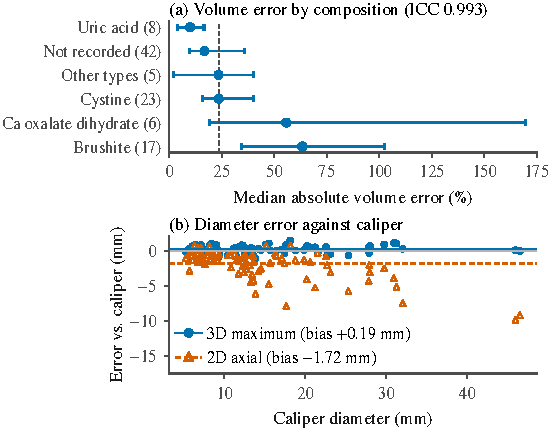
\includegraphics[width=0.567\columnwidth]{figures/fig2_phantom.pdf}
\caption{Physical reference (Freiburg, 101 stones). (a) Median absolute per-stone volume error by recorded composition (number of stones; bootstrap 95\% CIs; dashed line, all stones, 23.6\%) at a volume ICC of 0.993. (b) Automated diameter minus caliper diameter for the 3D maximum (filled) and the 2D axial maximum (open); lines: bias. 7 stones are in the correct 10\,mm category only by 3D ($p=0.016$).}
\label{fig:phantom}
\end{figure}

\subsection{Protocol and statistics}
Before the calibration and test scans were unlocked, we hashed and committed the protocol, code, configuration, model checkpoint and split. The calibration quantities were hashed before the test scans were loaded, and the evaluation was run once. There was a single formal test (nominal 0.90, filter on) with two criteria. The paired median width ratio of the burden interval to P2-B-CQR (the median over scans of each scan's width ratio) had to have a scan-level paired percentile-bootstrap 95\% CI below 1 (10{,}000 resamples, fixed seed), and the Clopper--Pearson upper bound of its coverage had to be at least 0.90. This is not a non-inferiority test. We estimated beforehand how often it would pass, using a development-only simulation of the locked design (200 seeded development splits of 77 fitting, 35 pseudo-calibration and 53 pseudo-test scans). Both criteria were met in 64\% of repetitions and the coverage criterion alone in 99.5\%; without the filter, both were met in 71.5\%. A negative locked result was therefore quite possible. A pre-specified power simulation gave under 80\% power for per-stone coverage on 53 scans, so we treat per-stone results as descriptive. Sensitivity cohorts S1 and S2 removed scans flagged by a non-radiologist screening review (S1: exclusions; S2: all flags) from all sets; S3 removed locked scans in cross-split suspected repeat pairs from calibration and test. Scan-level coverage CIs are Clopper--Pearson. Per-stone CIs in the text resample scans (10{,}000 resamples), whereas the Clopper--Pearson bars of Fig.~\ref{fig:bands} assume independent stones; paired differences and ratios also resample scans. With one formal test and every other comparison descriptive, no multiplicity adjustment is applied. Some pre-specified descriptive endpoints were not produced by the single run and are not reported: per-stone coverage by annotated size, attenuation and slice group; scans with all stones covered by U2; calibration of $\pi$; agreement and Dice by size; and two further comparators.

\begin{table*}[t]
\caption{Locked test (53 scans, 11 of them stone-free): patient-burden intervals at nominal 0.90 with the pre-specified 30\,mm filter. Width ratio: paired median ratio to P2-B-CQR with scan-level bootstrap 95\% CI.}
\label{tab:t1}
\centering\footnotesize
\setlength{\tabcolsep}{3.5pt}
\begin{tabular}{lcccccc}
\toprule
Method & Coverage & Clopper--Pearson 95\% & Stone-free & Median width (mm$^3$) & Width ratio (95\% CI) & Formal test \\
\midrule
P2-0, naive sum of per-stone bounds & 36/53 (0.679) & 0.537--0.801 & 7/11 & 1{,}567 & -- & -- \\
P2-B, direct split conformal & 48/53 (0.906) & 0.793--0.969 & 8/11 & 30{,}369 & -- & -- \\
P2-B-CQR, conformalised quantile regr. & 49/53 (0.925) & 0.818--0.979 & 9/11 & 7{,}431 & 1 (reference) & -- \\
\textbf{Detection-aware (ours)} & \textbf{50/53 (0.943)} & 0.843--0.988 & \textbf{10/11} & \textbf{3{,}090} & \textbf{0.573} (0.540--0.656) & met \\
\bottomrule
\end{tabular}
\end{table*}

\section{Results}
\subsection{Agreement statistics hide stone-level error}\label{sec:res_phantom}
According to the fixed-threshold approach \cite{neubauer2023} used for the Freiburg phantom, the volume obtained reached an ICC(A,1) value of 0.993. However, the median absolute error of estimated stone volume was nevertheless found to be 23.6\% (95\% CI 17.1--38.4\%), with the error being 39.4\% for stones of 10--20\,mm size, and as per composition it ranged from 9.9\% ($n = 8$, uric acid) to 63.4\% ($n = 17$, brushite; Fig.~\ref{fig:phantom}a). Also, diameters were measured in comparison with the measurement carried out with the use of caliper, taking the definition of diameter according to \cite{neubauer2023} (maximum distance between voxel-centres plus 0.7\,mm). Thus, the diameter measured in 3D was found to be biased by 0.19\,mm (limits of agreement $-0.87$ to $+1.25$\,mm), while the 2D axial diameter measured was found to be $-1.72$\,mm ($-5.67$ to $+2.22$\,mm). Seven stones were correctly classified at the 10\,mm threshold only in the case when measurements have been performed in 3D but not in 2D, and none only in 2D (exact McNemar $p = 0.016$, descriptive; Fig.~\ref{fig:phantom}b). In the annotations of the development-set, 11.3\% of the stones had been classified into different size categories when going from 2D to 3D.

\subsection{Confirmatory burden result}
Both formal conditions were satisfied (see Table~\ref{tab:t1}). The detection-aware interval covered 50 out of the total 53 scans (0.943; Clopper--Pearson 0.843--0.988). The median width of the interval equaled 3{,}090\,mm$^3$ while that of P2-B-CQR was 7{,}431\,mm$^3$. The median of the paired width ratios was 0.573 (0.540--0.656). There was no detectable difference in coverage between the presented method and P2-B-CQR (paired differences $+0.019$; 95\% CI $-0.057$ to $+0.094$). Hence, the improvement is a narrower interval that ensures similar coverage but not better coverage. The method ensured covering 10 out of 11 scans without stones. The post-hoc replay of the testing process helped to explain where the advantage of the presented method came from. The ratio of the scans containing stones was 0.554 (0.535--0.609), which is narrower for 36 out of the total 42 cases. The method was wider for the scans without stones, where the median equaled 710\,mm$^3$ as opposed to the 32\,mm$^3$.


\begin{figure*}[t]
\centering
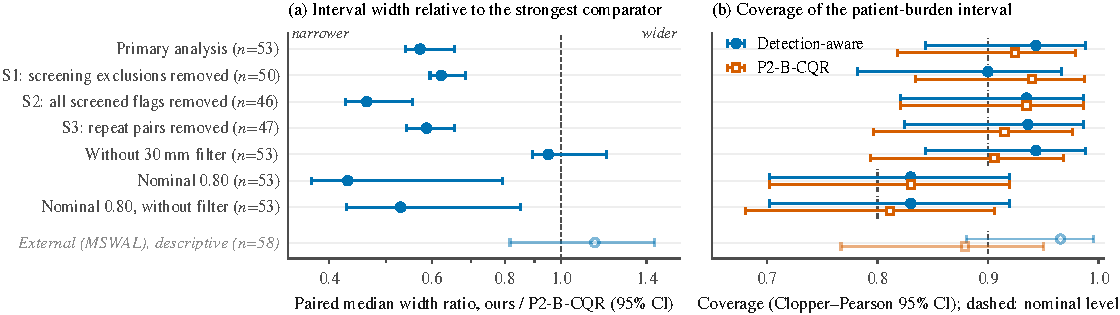
\includegraphics[width=0.579\textwidth]{figures/fig3_burden_robustness.pdf}
\caption{Sensitivity analyses and external check of the burden result (nominal 0.90 unless stated). (a) Paired median width ratio of the detection-aware interval to P2-B-CQR with scan-level bootstrap 95\% CI; values below 1 mean narrower intervals. (b) Patient-level coverage with Clopper--Pearson 95\% CIs for both methods. Rows: the primary locked-test analysis, the pre-specified sensitivity cohorts S1--S3, the filter ablation, the descriptive nominal-0.80 analyses, and the external check (descriptive; no refitting). Dashed ticks mark each row's nominal level.}
\label{fig:forest}
\end{figure*}

The benefit was present in three groups that were specified beforehand (see Fig.~\ref{fig:forest}). The ratios of the width were 0.622 (S1; 50 test scans), 0.464 (S2; 46) and 0.588 (S3; 47) and all conditions were met for them. The coverage in the S1 cohort was equal to 0.900 (45 out of 50). Without the 30\,mm filter the ratio was 0.951 (0.893--1.194). This was not because our interval changed much (Table~\ref{tab:ablation}); the CQR comparator narrowed from 7{,}431 to 3{,}803\,mm$^3$. Post hoc, the comparator narrowed in all 43 test scans whose kept pieces were the same with and without the filter, so the change came from its fitting and calibration rather than from the test scans' pieces: its conformal correction from the 35 calibration scans was 1.29 (log scale) with the filter and 0.53 without. At nominal 0.90, the width advantage is therefore specific to the pre-specified filtered arm. At nominal 0.80 (descriptive) the ratio was 0.430 (0.373--0.792) with the filter and 0.531 (0.429--0.851) without it.

\subsection{Size-stratified per-stone intervals}
Research included 147 matching stones using 35 test scans. With respect to stone volumes, Mondrian intervals indicated coverage of 0.966 (0.926--0.993) with a relative width of 2.32 median. For the 3D stone diameters, the coverage was indicated at 0.952 (0.914--0.982) with a relative width of 1.06 median (see Fig.~\ref{fig:bands}). The standard global conformal interval lost coverage for stones estimated as being less than 5\,mm (31 stones, 16 scans); in terms of stone diameters, U1 provided coverage for 19 of the 31 stones (0.613; 0.400--0.784), U2 showed coverage for 29 stones (0.935; 0.800--1.000) and standard Bland--Altman coverage limits used provided coverage of 0.774. For volume measurement, the coverage rates turned out to be as follows: U1 (0.806), U2 (0.935) and the much wider Bland--Altman limits also 0.935 (median relative width 3.80). The exploratory method U4 that showed narrower width showed similar coverage (see tab.~\ref{tab:ablation}; below 5\,mm: volume 0.968, diameter 0.935). We had first seen the same pattern in the OOF development data (465 stones; volume below 5\,mm: U1 0.734, U2 0.879), so the held-out result replicates a development observation.

\begin{figure}[t]
\centering
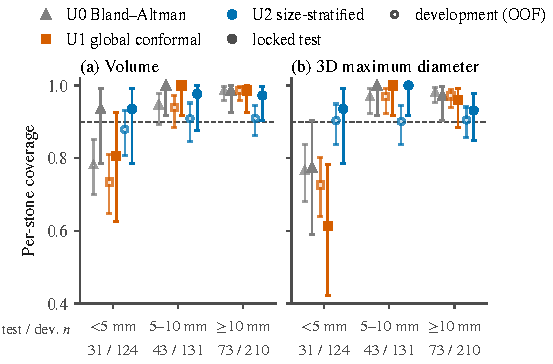
\includegraphics[width=0.567\columnwidth]{figures/fig4_size_bands.pdf}
\caption{Per-stone coverage by predicted-size band at nominal 0.90 (dashed line) for Bland--Altman limits (U0), a global conformal interval (U1) and the size-stratified interval (U2). Filled markers: locked test; open markers: out-of-fold development. Bars: Clopper--Pearson 95\% CIs (independent stones assumed). Below each band: number of test / development stones.}
\label{fig:bands}
\end{figure}

\subsection{Factors that affect intervals}
Other variations of development are included in Table~\ref{tab:ablation}. When missed burden factors are excluded, the coverage drops from 0.915 to 0.879, and the interval increases considerably from 1{,}530 to 2{,}002\,mm$^3$. However, the confidence intervals (CIs) intersect with one another, which is consistent with those missed stones accounting for only 1.9\% of the burden. By making changes in the false-positive model, we managed to keep the coverage stable although the interval increased by 11\% at median. Two models where we took each stone separately were not useful for withheld data. The first one was an asymmetric interval design that came up after we saw that 45 out of 46 development misses were under-estimates, however, this interval was much wider in the withheld data set. The other one that provided joint volume measures for all the stones of a patient \cite{andeol2025} proved unhelpful. In the development stages, U2 volume intervals had the highest misreporting in the lowest attenuation 16.8\% and lowest elongation 14.8\% groups.

\begin{table}[t]
\caption{Ablations and exploratory variants (nominal 0.90), all descriptive. Dev.: out-of-fold development; Test: locked test, secondary or exploratory analyses (the confirmatory result is Table~\ref{tab:t1}).}
\label{tab:ablation}
\centering\footnotesize
\setlength{\tabcolsep}{3pt}
\begin{tabular}{lccc}
\toprule
Variant & Data & Coverage & Width \\
\midrule
\multicolumn{4}{l}{\emph{Burden interval (width in mm$^3$)}} \\
Detection-aware & Dev. & 0.915 & 1{,}530 \\
\quad no missed term & Dev. & 0.879 & 2{,}002 \\
\quad distance-only FP$^{a}$ & Dev. & 0.925 & +11\% \\
\quad no 30\,mm filter & Test & 0.943 & 3{,}335 \\
P2-B-CQR, no filter & Test & 0.906 & 3{,}803 \\
\midrule
\multicolumn{4}{l}{\emph{Per-stone interval (median relative width)}} \\
U2, vol./diam. & Test & 0.966/0.952 & 2.32/1.06 \\
Asymm.\ U2$^{b}$ & Test & 0.912/0.966 & 23.9/2.32 \\
U4, vol./diam.$^{c}$ & Test & 0.952/0.939 & 1.58/0.56 \\
Joint, volume & Test & 1.000 & 44.5 \\
\bottomrule
\multicolumn{4}{l}{\scriptsize $^{a}$Median per-split change, 200 dev.\ splits. $^{b}$Post hoc. $^{c}$Exploratory, TTA-scaled.}
\end{tabular}
\end{table}

\subsection{External check}
From the total of 77 stone-bearing MSWAL scans, 58 were performed without any contrast and 19 scans were with the contrast agent. None of them failed to be processed. We used the frozen system and calibration without the need for any refitting (refer to Table~\ref{tab:external}). The level of burden coverage remained satisfactory (since it was 56 out of 58), but the detection-aware interval was no longer narrower than P2-B-CQR (ratio = 1.142; 0.817--1.444). The measure of coverage in terms of the diameter per stone remained quite close to what it should have been (0.893); however, in terms of the measure of coverage based on the volume, values dropped down to the level of 0.733 (0.625--0.831). The global U1 covered even less. The case mix also differed: 51\% of matched MSWAL stones were predicted below 5\,mm, against 21\% in the Li test set, and few small annotated stones were detected. These results are descriptive, and with one external dataset we cannot separate differences in annotation convention from model error.



\begin{table}[t]
\caption{Locked test (Li 2022) versus external check (MSWAL), frozen system and calibration, nominal 0.90.}
\label{tab:external}
\centering\footnotesize
\setlength{\tabcolsep}{2.5pt}
\begin{tabular}{lcc}
\toprule
 & Li test & MSWAL \\
\midrule
Scans analysed & 53 & 58 of 77 \\
Burden coverage & 50/53 (0.843--0.988) & 56/58 (0.881--0.996) \\
Width ratio vs.\ CQR & 0.573 (0.540--0.656) & 1.142 (0.817--1.444) \\
U2 vol./diam.\ coverage & 0.966/0.952 (147) & 0.733/0.893 (75) \\
U1 vol./diam.\ coverage & 0.952/0.898 & 0.520/0.587 \\
False positives per scan & 0.78$^{\dagger}$ & 0.79 \\
Stones predicted $<$5\,mm & 21\% & 51\% \\
Detected by size$^{\ddagger}$ & 18/52/76/93\%$^{\dagger}$ & 3/23/81/95\% \\
\bottomrule
\multicolumn{3}{l}{\scriptsize $^{\ddagger}$Annotated $<$3 / 3--5 / 5--10 / $\ge$10\,mm. $^{\dagger}$OOF development, 165 scans.}
\end{tabular}
\end{table}

\section{Limitations}
The patient reference standard is a single-centre annotation rather than physical reality. The annotations highlighted through our screening were not validated by a radiology professional, so no sensitivity tests using confirmed reading errors were carried out. The results are based on a locked test set comprising 53 scans and one model fold. There could still have been patient leakage beyond the S3 repetitions. The per-stone intervals refer only to the stones which can be detected and are not calibrated for attenuation on a conditional basis. Per-stone intervals treat stones within a patient as exchangeable even though they are clustered \cite{dunn2023}; the per-stone CIs therefore resample whole scans. The phantom has no stones below 5\,mm and used a single scanning protocol. The external test used one dataset without phase data, and the transfer was incomplete. StoneKit is research software, hence the results cannot be used for actual diagnosis or clinical use.

\section{Conclusion and Future Work}
When using a method for automated measurement of kidney stones in a single locked evaluation, it was found that the detection-aware burden interval was narrower than that of a strong conformal baseline with similar coverage. The process of size stratification adds the possibility of improving the confidence in small-stone measurements. However, when using an external dataset, the advantage of the width of the interval was not preserved while the burden coverage was present. Before use at another centre, the quantiles $q_k$ should be recalibrated locally, especially for stones below 5\,mm. At the moment, we focus on the recalibration using local data as well as establishing references decided upon by readers and estimating the within-patient correlation of per-stone errors.

Currently, our software provides information on the size of the stones but does not specify their location within the kidney or surrounding anatomy. We feel it is necessary to make several improvements. The first one is to localize each stone while specifying its size, surface distance, and associated anatomical features around the stones. The second stage would entail the measurement of changes happening to the anatomy of the kidney through comparing both kidneys from the patient and checking the dilation of the collecting system, thickness of the parenchyma, and asymmetry of kidney volume. Third, relate these changes to stone size, burden and location, and examine which changes appear already at small burden. Single scans can show associations only; an order of changes needs repeat scans of the same patients, or has to be inferred with an explicit disease-progression model and reported as such.

\noindent\textbf{Acknowledgment and source of financing.} The authors express gratitude to Dr.~Suresh Kumar Kanaparthi (Department of Computer Science and Engineering, SRM University-AP; sureshkumar.k@srmap.edu.in), their supervising mentor, for valuable advice during the course of the project. No external financing for the completion of the research has been acquired. \textbf{Availability of data and program code.} The CT images of the patients are available from the original authors via Zenodo (doi:\,\url{10.5281/zenodo.6042410}); redistribution of the data is not possible in this context. The data obtained from the physical reference phantom (CC BY 4.0; doi:\,\url{10.6084/m9.figshare.21992264}) and MSWAL dataset (CC BY-NC 4.0) can be accessed from the sources indicated in \cite{neubauer2023}, \cite{wu2026mswal}. The programming code (including the workstation) as well as configurations, frozen protocols, the respective hash manifest, aggregated files with the results and graphs compiled in each table or figure can be found on \url{https://github.com/SaiPraneeth9955/stonekit}; all the materials provided can be used according to MIT licence. Model weights trained on the patient data are not distributed.

\renewcommand{\footnotesize}{\scriptsize}
\bibliographystyle{IEEEtran}
\bibliography{references}
\end{document}
